% !TeX root = ../main.tex

\chapter{动机和背景}
\label{chap:background}

本章将介绍本研究的动机和相关背景。
\autoref{sec:bg-perf-isolation}将介绍云闪存系统中的多组合性能隔离问题重要性,
以及SSD的读写干扰问题及其产生的原因。
\autoref{sec:bg-related-work}将分别从硬盘本身和系统设计的层面介绍改进SSD存储系统服务质量的相关工作。

\section{云闪存系统中的多租户性能隔离问题}
\label{sec:bg-perf-isolation}

基于NAND介质闪存具有低延迟、高吞吐的特点,给存储系统带来了革命性的影响。
但是,对于云系统来说,只有当它能够稳定、可预测地提供以上特点时,基于闪存的SSD才能得到利用。
现代的虚拟化技术使得云系统中的多个租户可以共享同一个物理资源,却给每个租户独占该资源的假象~\cite{bugnion2017hardware}。
在这种抽象中,各个租户间的性能隔离对于满足租户的服务质量要求至关重要~\cite{somani2009isolation}。
若云系统的性能隔离不够充分,则每个租户随时可能受到其“吵闹的邻居”(Noisy Neighbor)的影响,其性能的稳定性将会受损。

在存储系统中,性能隔离主要指的是任一租户对物理资源访问的带宽和延迟基本不受其他租户的影响。
由于机械硬盘的延迟普遍较差,且读写性能差异不大,因此限制各个租户的带宽往往就可以实现多租户的性能隔离。
例如,Docker通过Linux的cgroup~\cite{cgroup}设置每个租户的带宽上限;
Ceph~\cite{weil2006ceph}也通过mClock~\cite{gulati2010mclock}设置虚拟时间,限制每个租户发送请求的频率,从而实现分布式的租户资源限制。

然而,交互性高的数据应用服务需要良好的存储尾延迟保证~\cite{dean2013tail,hao2016tail}。
这是因为现代云系统的分布式和并发特性,使得一个Web请求往往被同时分发到多个服务器上分别处理,该Web请求的响应时间将是这多个服务器的服务时间的最大值。
因此,若一个服务器响应时间的99\%分位数为2ms,则若一个请求被分发到100个服务器上处理,其响应时间的$0.99^{100}=36.6\%$分位数将为2ms。
也就是说,超过60\%的Web请求将经历尾延迟。
因此,某些用户除了对访问带宽有要求,还会要求对自己租用的SSD的读请求中99\%均有两毫秒以下的延迟。
尽管可以通过设置不同租户的优先级保证某些租户的请求被优先服务,但并不能给出严格的尾延迟保证。
在这种情况下,仅仅对每个用户的访问带宽进行限制是不够的。

\begin{figure}[h]
  \centering
  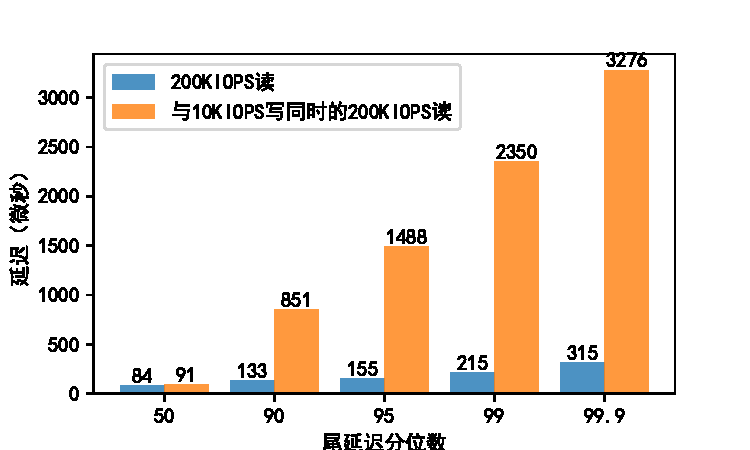
\includegraphics[width=0.8\textwidth]{thesis-wr-interfere.pdf}
  \caption{写操作对其他租户读延迟的影响。很小的写吞吐就使读租户的尾延迟增大了约10倍。}
  \label{fig:bg-wr-interfere}
\end{figure}

SSD内部的\textit{读写干扰}使多租户的性能隔离更加复杂。
对SSD的写操作可能会引起SSD内部的垃圾回收、缓冲区刷新等操作。
由于SSD内部的存储采用日志结构~\cite{ArpaciDusseau18-Book},因此对SSD中存储页的修改或删除并不会立即改变该页的内容,而只是将其标记为不再使用。
垃圾回收指的就是将不再使用的页回收起来准备之后使用,并把仍在使用的页合并在一起的过程。
此外,SSD为了最佳的写吞吐,会在内部维护写缓冲区,只有当缓冲区写满时才会将数据写入存储介质中。
缓冲区刷新指的就是上述写入存储介质的过程。
由于上述两种行为涉及对SSD内部的操作,因此同时进行的其它读写操作往往会被阻塞。

如\autoref{fig:bg-wr-interfere}所示,当一个租户在进行读操作时,另一个租户对不同位置的写操作是该租户的尾延迟增大了约十倍。
这就是由于上文提到的写操作触发的SSD内部的垃圾回收、缓冲区刷新等行为引起的。
当某个租户进行写操作时,SSD内部可能会进行针对某一区域的垃圾回收或缓冲区刷新,这些活动将会对该硬盘上其他租户的访问性能造成影响。
尽管这些活动并不常见,但这些异常的延迟却构成了租户的尾延迟。

\section{相关工作}
\label{sec:bg-related-work}

本节介绍在云闪存系统中提供服务质量保证的相关工作。
\autoref{sec:bg-related-work-ssd}将介绍如何在SSD层面提供服务质量的保证,
\autoref{sec:bg-related-work-system}将介绍在系统层面提供服务质量保证的方法。

\subsection{保证服务质量的SSD}
\label{sec:bg-related-work-ssd}

在SSD层面上提供服务质量的方式主要可分为两种。
第一种是对SSD的性能进行建模,从而预测垃圾回收、写缓冲区刷新等操作会在何时发生。
SSDCheck~\cite{kim2018ssdcheck}和FusionRAID~\cite{jiang2021fusionraid}通过一系列测试IO请求序列来获取SSD的垃圾回收间隔、写缓冲区大小等信息,
但是他们的测试脚本都基于对SSD行为的假设,在我们的实验中,并非所有SSD都遵循这一假设;
除此之外,ReFlex~\cite{klimovic2017reflex}利用曲线拟合,为SSD上的读写请求设定权重,后续每个租户的加权IOPS不能超过为其设定的限制;
近期,LinnOS~\cite{hao2020linnos}通过一个轻量的神经网络来预测每个请求的延迟是否会较大。

另一种方法是修改SSD控制器,使其具有控制服务质量的特性。
例如,NVMe 1.4标准~\cite{nvme2020}提出了I/O Determinism和NVM Set。
其中,I/O Determinism提供了具有确定性延迟和不确定性延迟的时间窗口,它规定了用户与SSD之间的一种协议。
SSD保证在确定性窗口中不进行后台的维护操作,用户则保证在确定性窗口中不进行写操作~\cite{petersen2018enabling}。
NVM Set是在SSD控制器层面就将资源拆分为多个集合,从而支持多个租户无干扰地共享同一SSD。
此外,还有其它通过修改SSD控制器~\cite{yan2017tiny,arash2018flin}和使用Open-Channel SSD来改进SSD的尾延迟的方法。

\subsection{保证服务质量的云服务系统}
\label{sec:bg-related-work-system}

如\autoref{sec:bg-perf-isolation}所述,传统的云存储服务大多以保证租户的吞吐为服务质量的优化目标~\cite{patterson2004latency, cgroup,gulati2010mclock}。
近年来,尾延迟越来越受到重视~\cite{dean2013tail},确保低尾延迟的一种常用方法是利用冗余。
% \JF{Performance Variablity?}

利用冗余的方法之一是负载均衡,即将每个请求尽可能分到负载最低的机器上,从而获得最好的响应时间。
有大量研究通过推断各个冗余服务器的负载来进行尽可能最优的请求分发。
例如,C3~\cite{suresh2015c3}通过估计队列深度和服务时间对冗余服务器进行排序来选择最优的冗余服务器。
\autoref{sec:bg-related-work-ssd}提到的对SSD进行性能建模的方式也可以用来进行冗余服务器的选择。

另一种利用冗余的方法是hedging,即将同一请求同时发给多个冗余服务器,并以其中最快的一个作为最终的结果。
在这种情况下,只有当所有冗余服务器均出现尾延迟时,该请求才会出现异常的高延迟,因此能将异常延迟出现的可能大大降低。
然而,这种方法会使各个服务器的负载增加~\cite{primorac2021hedge},因此并不能在所有情况下都确保比不使用冗余的尾延迟更好。
\citet{vulimiri2013low}通过排队论对利用冗余改善延迟进行了定量分析。

除此之外,还有一些系统试图在资源调度和集群管理时确保服务质量。
例如,PSLO~\cite{li2016pslo}利用控制论中的方法,实现了机械硬盘上的请求级尾延迟保证;
Quasar~\cite{delimitrou2014quasar}利用协同过滤预测租户所需的服务质量,并利用一个贪心算法选择最适合的资源配置方式。